\documentclass[12pt]{article}

\usepackage[utf8]{inputenc}
\usepackage[T1]{fontenc}
\usepackage[polish,provide=*]{babel}
\usepackage{lmodern}
\usepackage{amsmath}
\usepackage{latexsym,amsfonts,amssymb,amsthm,amsmath}
\usepackage{enumitem}
\usepackage{float}
\usepackage{hyperref}
\usepackage{graphicx}
\usepackage{subcaption}
\usepackage{booktabs}
\graphicspath{{./images/}}

\setlength{\parindent}{0in}
\setlength{\oddsidemargin}{0in}
\setlength{\textwidth}{6.5in}
\setlength{\textheight}{8.8in}
\setlength{\topmargin}{0in}
\setlength{\headheight}{18pt}

\title{}
\author{Kacper Kłos}

\begin{document}

\maketitle

W raporcie analizowaliśmy zachowanie kabla przy bardzo szybkich sygnałach. Wysyłaliśmy sygnały o napięciu 5 V mający 100 ns oraz 10 ns trwa zwiększenie napięcia z 0 do 5 V. Badamy dwa kable o wartości referencyjnej impedancji równej \(75 \, \Omega\). Wpierw wydłużając kabel badaliśmy jak zmienia się czas z jakim sygnał dochodzi z powrotem, orzymane wyniki pozwoliły wyznaczyć nam prędkości sygnału na \(v_{\mathrm{good}} = (9{,}892 \pm 0{,}032) \times 10^{7} \, \mathrm{m/s}\) oraz \(v_{\mathrm{bad}} = (11{,}341 \pm 0{,}080) \times 10^{7} \, \mathrm{m/s}\). Następnie na koniec kabla przyłożyliśmy opornik o zmiennym oporze i wyznaczyliśmy zależnść napięcia sygnału odbitego od oporu, przy pomocy tych wyników wyznaczyliśmy impedencję \(Z_{\mathrm{good}} = (73{,}9 \pm 1{,}1) \, \Omega\) oraz \(Z_{\mathrm{bad}} = (77{,}7 \pm 1{,}3) \, \Omega\). Na koniec przy pomocy tych wyników wyznaczyliśmy pojemność i indukcyjność na jednostkę długości kabla, wynoszące kolejno \(c_{\mathrm{good}} = (1{,}367 \pm 0{,}020) \times 10^{-10} \, \mathrm{F/m}\),  \(c_{\mathrm{bad}} = (1{,}135 \pm 0{,}021) \times 10^{-10} \, \mathrm{F/m}\), \(l_{\mathrm{good}} = (7{,}47 \pm 0{,}11) \times 10^{-7} \, \mathrm{H/m}\), \(l_{\mathrm{bad}} = (6{,}85 \pm 0{,}12) \times 10^{-7} \, \mathrm{H/m}\)

\newpage

\section{Wyniki Pomierów}
Wpierw badaliśmy czas potrzebny do odbicia sygnału dla kabla dobrego i złego z impedencją \(75 \, \mathrm{\Omega}\).

\begin{table}[H]
	\centering
	\begin{tabular}{c|cc|cc}
		\toprule
		\textbf{Nr} & \multicolumn{2}{c|}{\textbf{Dobry kabel}} & \multicolumn{2}{c}{\textbf{Zły kabel}}                      \\
		            & $d$ [m]                                   & $t$ [ns]                               & $d$ [m] & $t$ [ns] \\
		\midrule
		1           & 30                                        & 154                                    & 20      & 84       \\
		2           & 60                                        & 304                                    & 40      & 164      \\
		3           & 40                                        & 206                                    & 40      & 174      \\
		4           & 80                                        & 406                                    & 80      & 346      \\
		5           & 65                                        & 332                                    & 60      & 264      \\
		6           & 130                                       & 662                                    & 120     & 524      \\
		7           & 80                                        & 404                                    & 80      & 356      \\
		8           & 160                                       & 810                                    & 160     & 708      \\
		9           & --                                        & --                                     & 100     & 438      \\
		10          & --                                        & --                                     & 200     & 872      \\
		\bottomrule
	\end{tabular}
	\caption{Porównanie pomiarów odległości $d$ i czasu $t$ dla dobrego i uszkodzonego kabla.}
	\label{tab:good_vs_bad_cable}
\end{table}

\begin{figure}[H]
	\centering
	\begin{subfigure}{0.45\textwidth}
		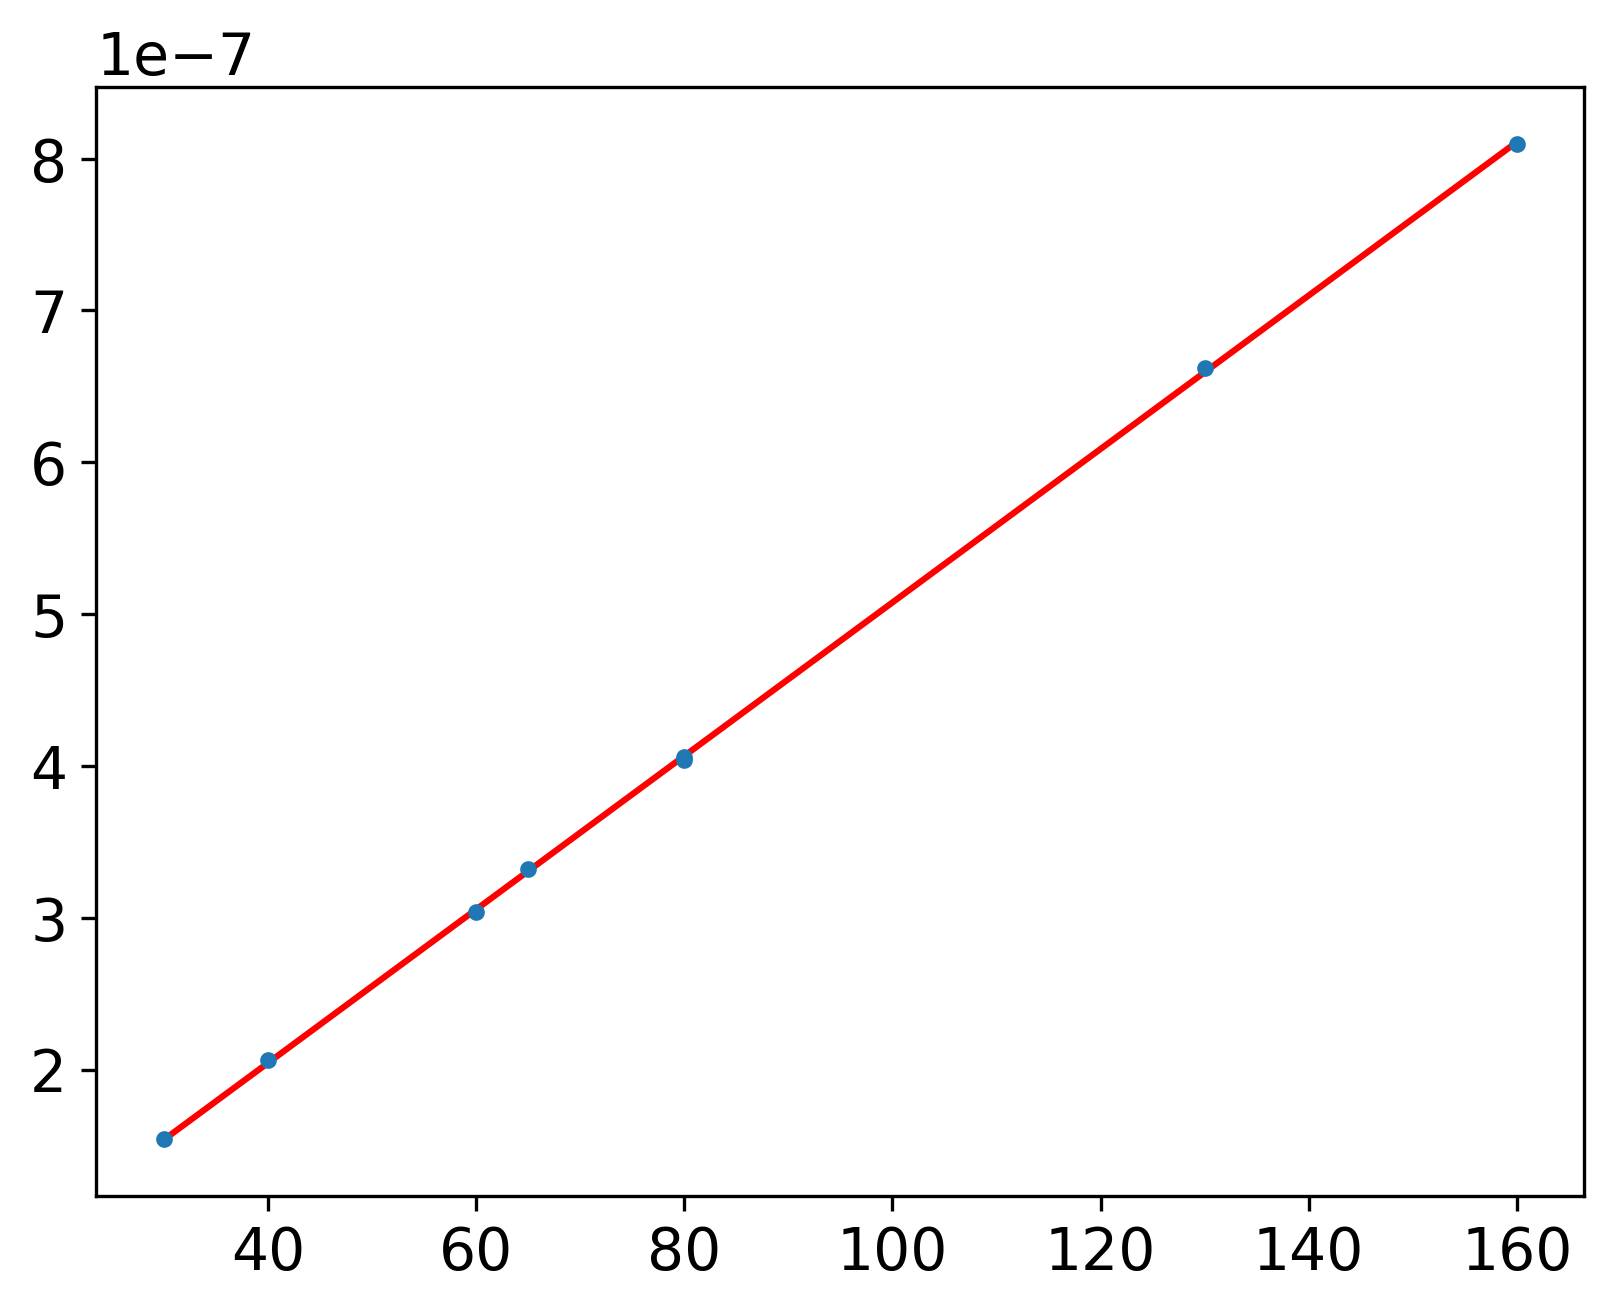
\includegraphics[width=\linewidth]{good_cable_distance}
		\caption{Dobry kabel}
		\label{fig:good_distance}
	\end{subfigure}\hfill
	\begin{subfigure}{0.45\textwidth}
		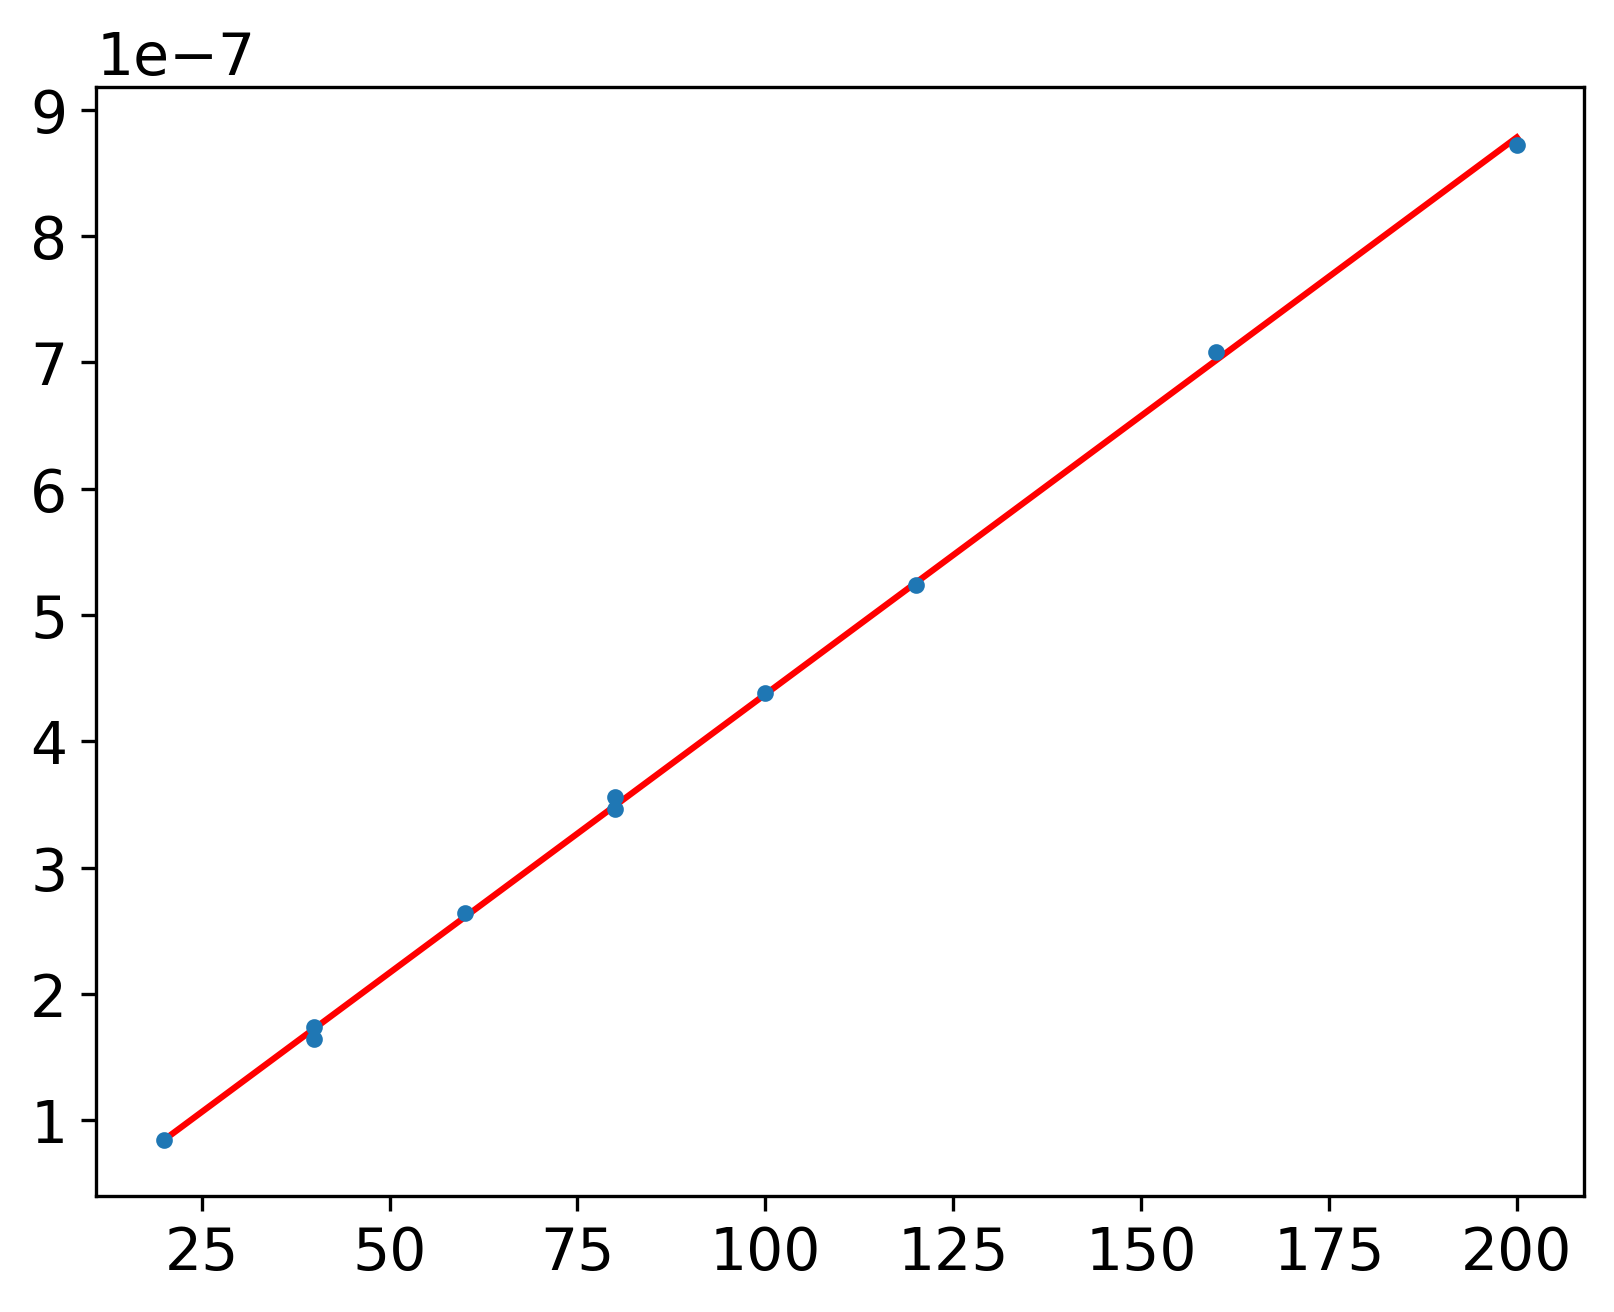
\includegraphics[width=\linewidth]{bad_cable_distance}
		\caption{Zły kabel}
		\label{fig:bad_distance}
	\end{subfigure}
	\caption{Wykres czasu między wysłanym a odebranym sygnałem \(t\) od długości kabla \(d\).}
	\label{fig:distance}
\end{figure}

Dopasowując prostą do danych (tab.~\ref{tab:good_vs_bad_cable}) i wzoru:
\[
	t = \frac{d}{v} + b
\]
otrzymujemy prędkość dla dobrago kable \(v_{\mathrm{good}}\) (fig.~\ref{fig:good_distance}) oraz dla złego \(v_{\mathrm{bad}}\) (fig.~\ref{fig:bad_distance})

\[
	v_{\mathrm{good}} = (9{,}892 \pm 0{,}032) \times 10^{7} \, \mathrm{m/s} \quad
	v_{\mathrm{bad}} = (11{,}341 \pm 0{,}080) \times 10^{7} \, \mathrm{m/s}
\]
Następnie mierzymy napięcie odbitego sygnały od oporu podłączonego do końca kabla.

\begin{table}[H]
	\centering
	\begin{tabular}{c|cc|cc}
		\toprule
		\textbf{Nr} & \multicolumn{2}{c|}{\textbf{Dobry kabel}} & \multicolumn{2}{c}{\textbf{Zły kabel}}                             \\
		            & $R$ [$\Omega$]                            & $U$ [V]                                & $R$ [$\Omega$] & $U$ [V]  \\
		\midrule
		1           & 21{,}242                                  & -1{,}200                               & 5{,}949        & -1{,}760 \\
		2           & 67{,}889                                  & -0{,}080                               & 21{,}741       & -1{,}160 \\
		3           & 51{,}489                                  & -0{,}400                               & 50{,}467       & -0{,}440 \\
		4           & 98{,}712                                  & 0{,}320                                & 73{,}712       & -0{,}040 \\
		5           & 154{,}450                                 & 0{,}800                                & 99{,}180       & 0{,}280  \\
		6           & 229{,}724                                 & 1{,}080                                & 154{,}913      & 0{,}680  \\
		7           & 346{,}970                                 & 1{,}400                                & 228{,}870      & 0{,}960  \\
		8           & 426{,}380                                 & 1{,}600                                & 324{,}130      & 1{,}200  \\
		9           & 502{,}590                                 & 1{,}680                                & 423{,}340      & 1{,}480  \\
		10          & 5{,}985                                   & -1{,}920                               & 502{,}510      & 1{,}520  \\
		\bottomrule
	\end{tabular}
	\caption{Porównanie pomiarów rezystancji $R$ i napięcia $U$ dla dobrego i uszkodzonego kabla.}
	\label{tab:good_vs_bad_cable_voltage}
\end{table}

\begin{figure}[H]
	\centering
	\begin{subfigure}{0.45\textwidth}
		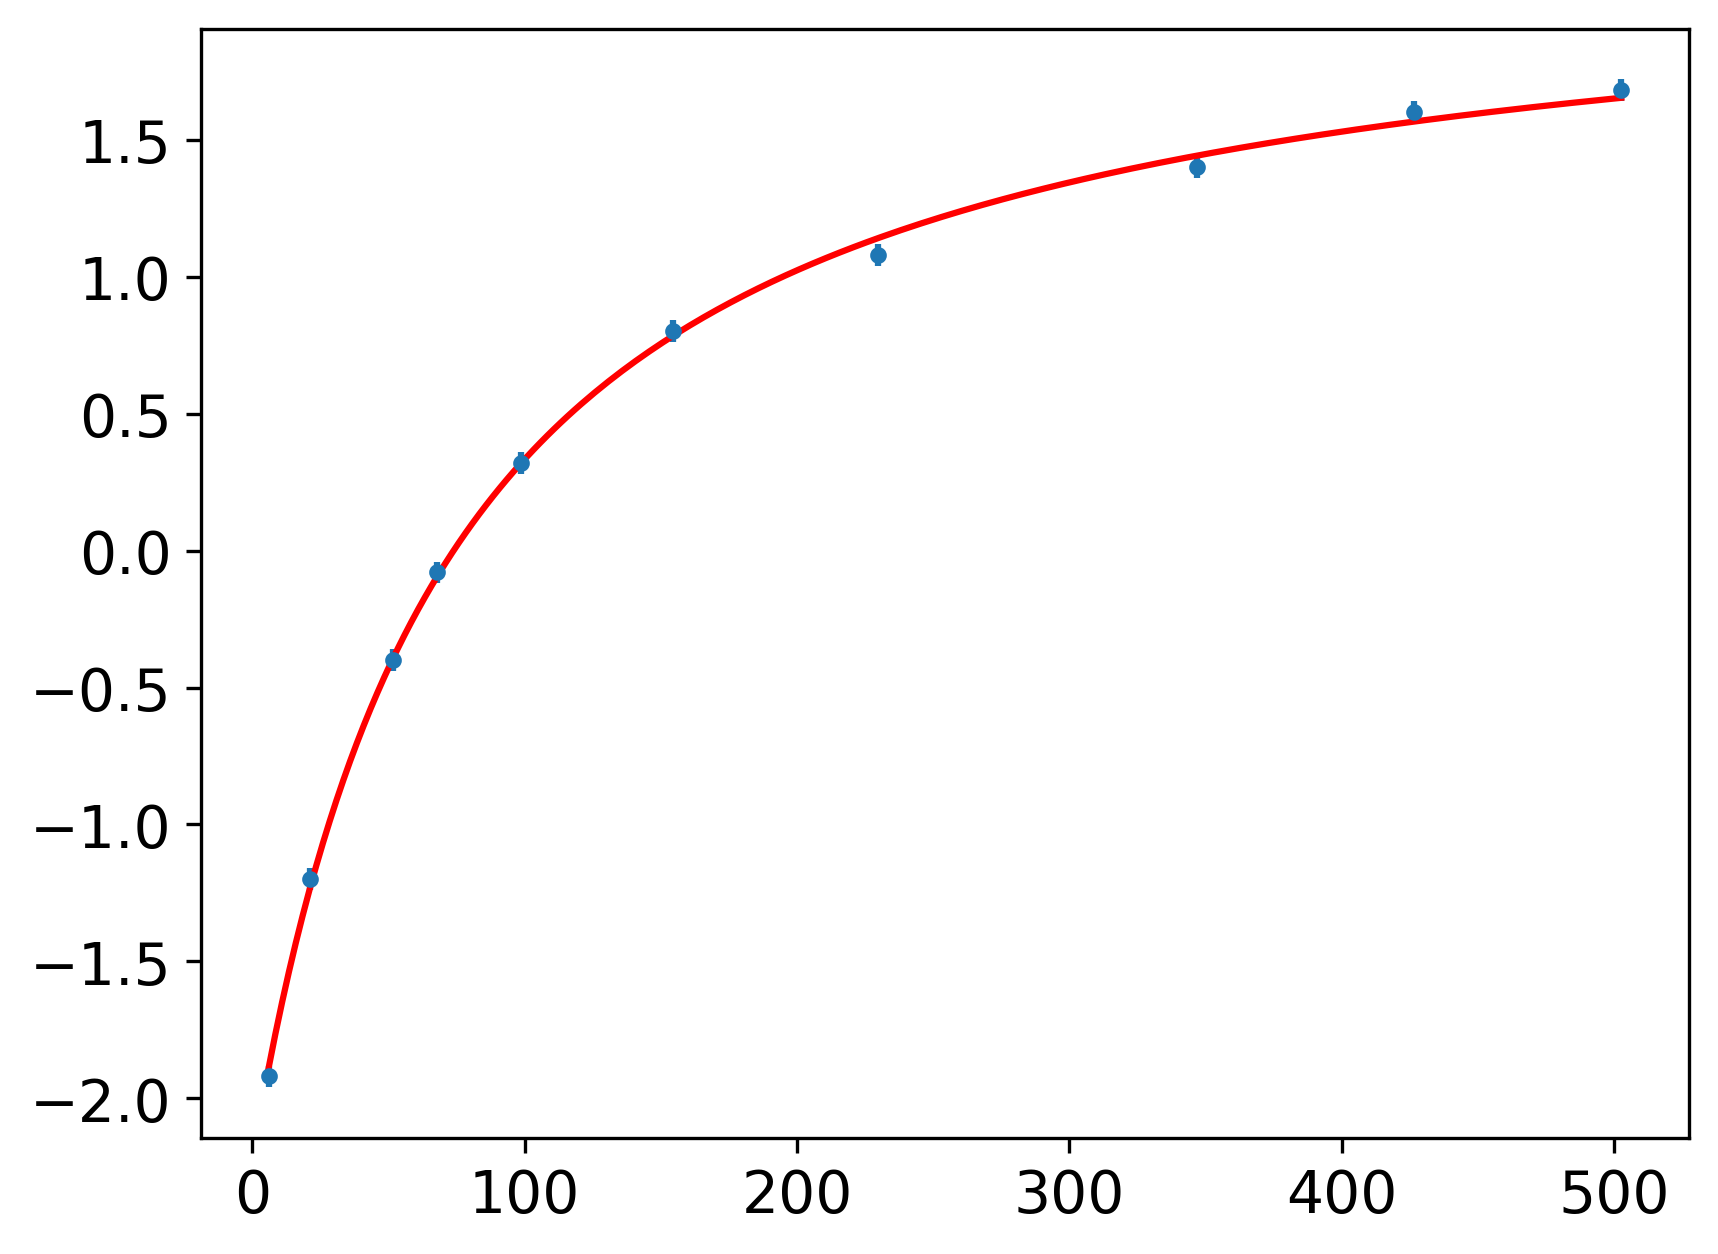
\includegraphics[width=\linewidth]{good_cable_voltage}
		\caption{Dobry kabel}
		\label{fig:good_voltage}
	\end{subfigure}\hfill
	\begin{subfigure}{0.45\textwidth}
		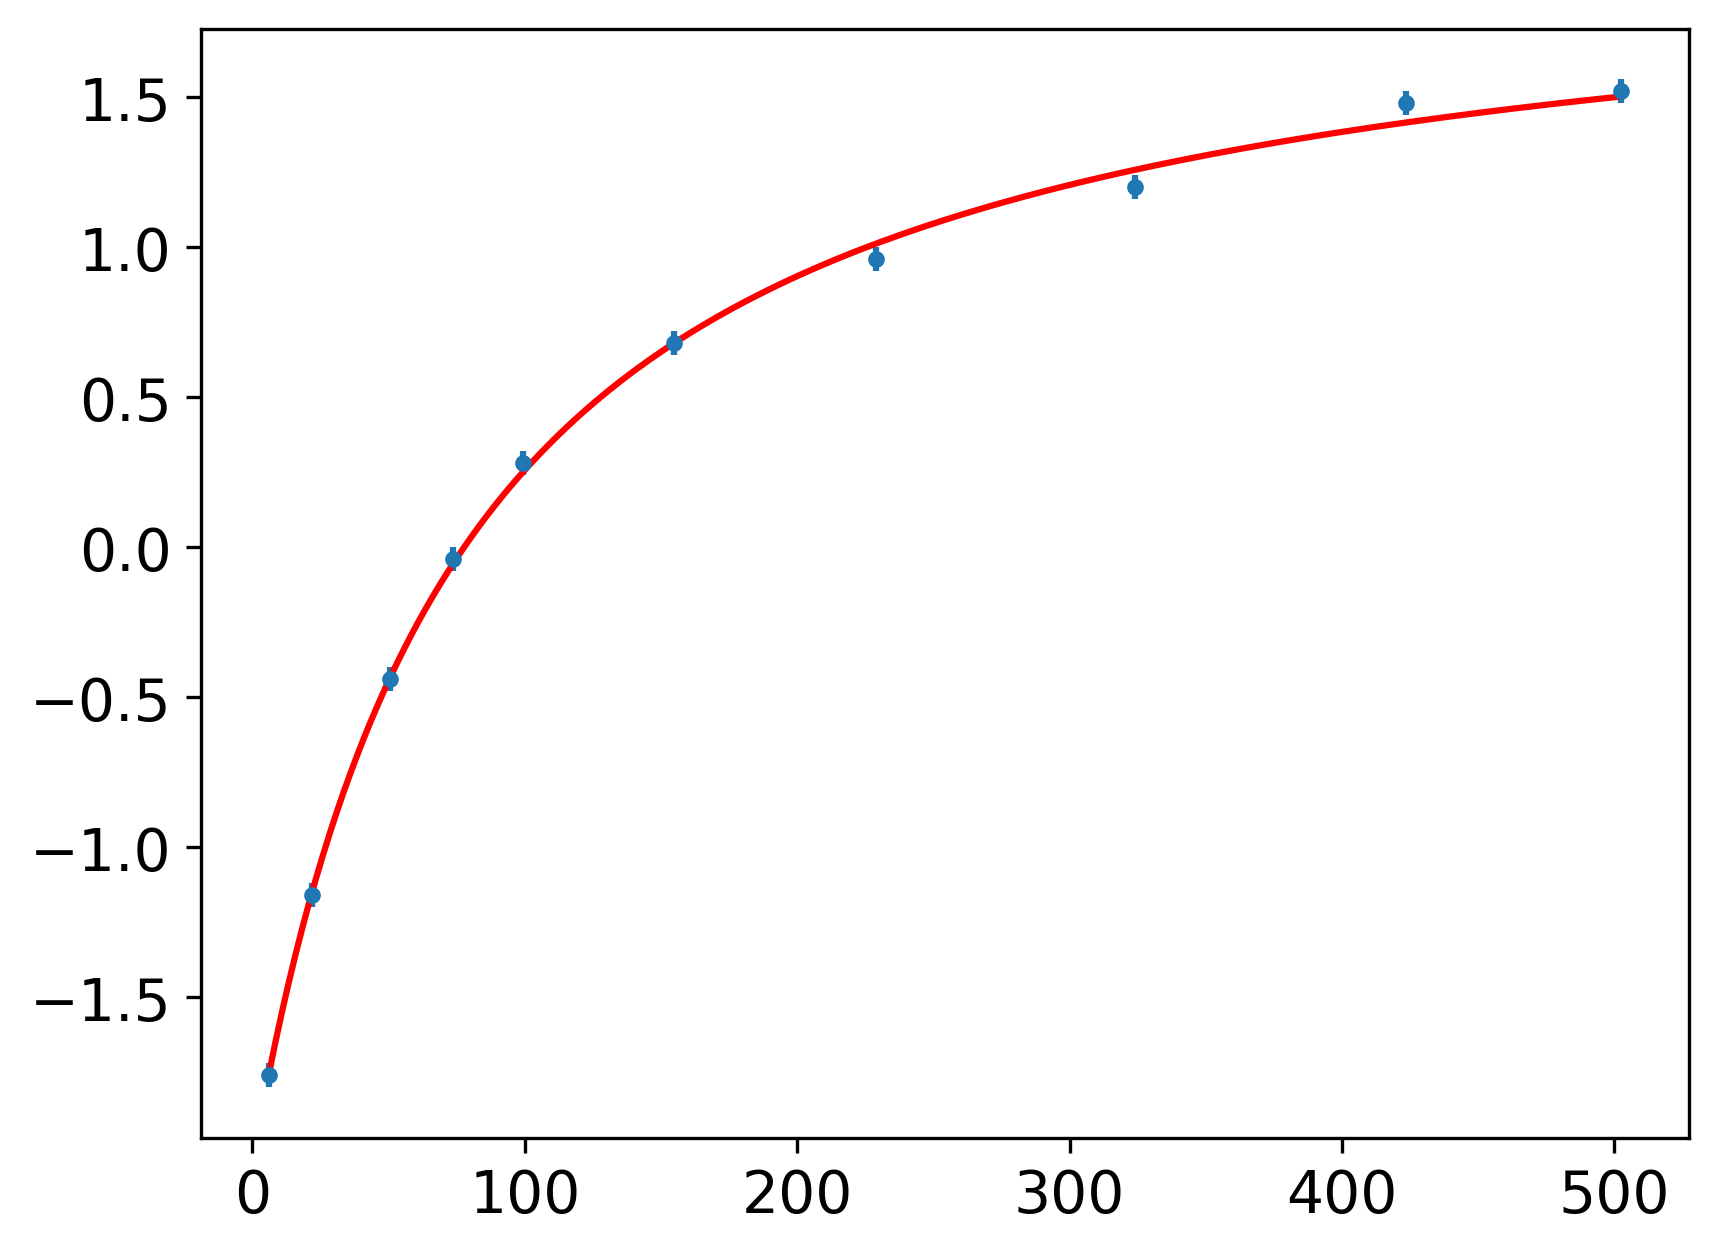
\includegraphics[width=\linewidth]{bad_cable_voltage}
		\caption{Zły kabel}
		\label{fig:bad_voltage}
	\end{subfigure}
	\caption{Wykres napięcia odbitego sygnału \(U\) od oporu na końcu przewodu \(R\)}
	\label{fig:distance}
\end{figure}

Dopasowując krzywą do wzoru otrzymanego w \cite{skrypt}:
\[
	U_1 = U_0 \frac{R_L - Z}{R_L - Z}
\]
Gdzie \(U_1\) - napięcie odbierane, \(U_0\) - napięcie generowane, \(R_L\) - opór opciążenia, \(Z\) - impedencja.

Oraz korzystając z otzymanych danych (tab.~\ref{tab:good_vs_bad_cable_voltage}) przy traktowaniu \(U_0\) i \(Z\) jako zmienną do której dopasowujemy otrzymujemy \(Z_{\mathrm{good}}\) (fig.~\ref{fig:good_voltage}) dla dobrego kabla i \(Z_{\mathrm{bad}}\) (fig.~\ref{fig:bad_voltage}) dla złego.
\[
	Z_{\mathrm{good}} = (73{,}9 \pm 1{,}1) \, \Omega \quad
	Z_{\mathrm{bad}} = (77{,}7 \pm 1{,}3) \, \Omega
\]
Korzystając z ponownie z wzorów obecnych w \cite{skrypt} możemy wyznaczyć pojemność \(c\) i indukcyjność \(l\) na jednostkę długości
\[
	c = \frac{1}{v Z} \quad l = \frac{Z}{v}
\]
Co przy naszych wartościach odpowiada:
\[
	c_{\mathrm{good}} = (1{,}367 \pm 0{,}020) \times 10^{-10} \, \mathrm{F/m} \, \quad l_{\mathrm{good}} = (7{,}47 \pm 0{,}11) \times 10^{-7} \, \mathrm{H/m}
\]
\[
	c_{\mathrm{bad}} = (1{,}135 \pm 0{,}021) \times 10^{-10} \, \mathrm{F/m} \, \quad l_{\mathrm{bad}} = (6{,}85 \pm 0{,}12) \times 10^{-7} \, \mathrm{H/m}
\]

\section{Analiza wyników}
Podczas badania mogliśmy zauważyć że sygnał wysyłany przez kabel zły znaczniej niż kabel dobry tłumił sygnały. W dodatku wyniki uzyskane przez kabel dobry miały mniejsze niepewności od tego złego, co skutkuje w tym że w przypadku impedencji wyznaczonych przez nas ta dla dobrego kabla mieści się w wartości referencyjnej \(75 \, \Omega\) podczas gdy wartość dla kabla złego, jest nieznacznie większa.

Jeśli mowa o błędzie to dla obu pomiarów błąd wynika z rozdzielczości oscyloskopu oraz generatora sygnałów. W przypadku pomiaru prędkości sygnału są to jedyne błędy, dlatego znajduje się on poniżej \(1 \%\) wyniku. Lecz w przypadku pomiarów napięcia błąd jest większy i wynika on głównie z trudności określenia dokładnego napięcia odbitego, które na przestrzeni czasu trwania odbitego sygnału spadało. Poza tym obecny jest niewielki błąd wynikający z rozdzielczości multimetra którym mierzyliśmy opór opornika na końcu kabla. Trzeba też wspomnieć że połączenia kabli mogły również zakłócić wyniki, jednak jest to pomijalne.

\begin{thebibliography}{1}

	\bibitem{skrypt}
	\emph{Kabel Koncentryczny}; Piotr Fita, Uniwersytet Warszawski.

\end{thebibliography}
\end{document}
